\documentclass[letterpaper]{article}
\usepackage[margin=1in]{geometry}
\usepackage[utf8]{inputenc}
\usepackage{textcomp}
\usepackage{amssymb}
\usepackage{natbib}
\usepackage{graphicx}
\usepackage{gensymb}
\usepackage{amsthm, amsmath, mathtools}
\usepackage[dvipsnames]{xcolor}
\usepackage{enumerate}
\usepackage{mdframed}
\usepackage[most]{tcolorbox}
\usepackage{csquotes}
% https://tex.stackexchange.com/questions/13506/how-to-continue-the-framed-text-box-on-multiple-pages

\tcbuselibrary{theorems}

\newcommand{\R}{\mathbb{R}}
\newcommand{\Z}{\mathbb{Z}}
\newcommand{\N}{\mathbb{N}}
\newcommand{\Q}{\mathbb{Q}}
\newcommand{\C}{\mathbb{C}}
\newcommand{\code}[1]{\texttt{#1}}
\newcommand{\mdiamond}{$\diamondsuit$}
\newcommand{\PowerSet}{\mathcal{P}}
\newcommand{\Mod}[1]{\ (\mathrm{mod}\ #1)}
\DeclareMathOperator{\lcm}{lcm}

%\newtheorem*{theorem}{Theorem}
%\newtheorem*{definition}{Definition}
%\newtheorem*{corollary}{Corollary}
%\newtheorem*{lemma}{Lemma}
\newtheorem*{proposition}{Proposition}


\newtcbtheorem[number within=section]{theorem}{Theorem}
{colback=green!5,colframe=green!35!black,fonttitle=\bfseries}{th}

\newtcbtheorem[number within=section]{definition}{Definition}
{colback=blue!5,colframe=blue!35!black,fonttitle=\bfseries}{def}

\newtcbtheorem[number within=section]{corollary}{Corollary}
{colback=yellow!5,colframe=yellow!35!black,fonttitle=\bfseries}{cor}

\newtcbtheorem[number within=section]{lemma}{Lemma}
{colback=red!5,colframe=red!35!black,fonttitle=\bfseries}{lem}

\newtcbtheorem[number within=section]{example}{Example}
{colback=white!5,colframe=white!35!black,fonttitle=\bfseries}{def}

\newtcbtheorem[number within=section]{note}{Important Note}{
        enhanced,
        sharp corners,
        attach boxed title to top left={
            xshift=-1mm,
            yshift=-5mm,
            yshifttext=-1mm
        },
        top=1.5em,
        colback=white,
        colframe=black,
        fonttitle=\bfseries,
        boxed title style={
            sharp corners,
            size=small,
            colback=red!75!black,
            colframe=red!75!black,
        } 
    }{impnote}
\usepackage[utf8]{inputenc}
\usepackage[english]{babel}
\usepackage{fancyhdr}
\usepackage[hidelinks]{hyperref}

\pagestyle{fancy}
\fancyhf{}
\rhead{CSE 131}
\chead{Monday, May 15, 2023}
\lhead{Lecture 18}
\rfoot{\thepage}

\setlength{\parindent}{0pt}

\begin{document}

\section{Garbage Collection (Continued)}
We will now discuss an algorithm that we can use to perform garbage collection. This algorithm is known as the \textbf{mark-compact algorithm}.

\subsection{Layout and Notation}
In the following sections, we'll make use of the following box to represent heap space. Each square box represents one word in the heap (so each group of boxes represents three words of contiguous heap memory).
\begin{center}
    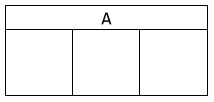
\includegraphics[scale=0.7]{../assets/GCAlgLayout.png}
\end{center}
The (A) represents an address to this group of memory (like \code{0x100}).

\bigskip 

The first box of each group is some metadata that we'll need for garbage collection. For our algorithm here, we will need to make use of this metadata. However, there are algorithms out there that don't require metadata.

\bigskip 

In any case, the important thing to remember is that, under this representation, \textbf{each pair} requires 3 words in the heap. 

\subsection{The Algorithm}
At a high level, our algorithm looks like 
\begin{verbatim}
    mark(roots):
        for ref in roots:
            mark_heap(ref)
    
    mark_heap(r):
        if r.marked:
            return 
        r.marked = true 
        for (i, r') in r:
            if ispair(r')
                mark_heap(r')

    fwd_headers():
        from = 0
        to = 0
        while move_from < HEAPEND:
            if from.marked: 
                from.fwd = to 
                to += 3 words/from.size 
            from += 3 words/from.size 
    
    fwd_internal(roots):
        for ref in roots:
            update_fwd(ref)
            fwd_heap(ref)

    fwd_heap(r):
        if r.fwded: 
            return 
        r.fwded = true 
        for (i, r') in r:
            if ispair(r')
                r[i] = getfwd(r')
                fwd_heap(r')

    compact():
        ... \end{verbatim}
Roughly speaking, we can break each of these methods into four groups: 
\begin{enumerate}
    \item \code{mark(roots)} and \code{mark\_heap(r)}
    \item \code{fwd\_headers()}
    \item \code{fwd\_internal(roots)} and \code{fwd\_heap(r)} (forwarding the internal pointers)
    \item Compacting.
\end{enumerate}

\subsection{Motivating Example}
Let's consider the following heap structure.
\begin{center}
    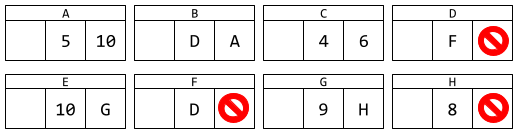
\includegraphics[scale=0.8]{../assets/GCAlg1.png}
\end{center}
Note that this example doesn't correspond to any particular program. 

\subsubsection{Step 1: Finding the Root Set}
\begin{mdframed}
    First, we want to find all the references that are currently on the stack (or registers). These are called the \textbf{root set}.
\end{mdframed}
Right now, we don't know what is considered garbage (since we don't know what the stack or the registers look like). So, let's suppose $G$ and $B$ are the only two references on the stack (or registers, depending on implementation). We call this the root set (the roots of your traversal into the heap). Let's suppose we want to \emph{clean} the heap. 

\subsubsection{Step 2: Marking Heap to Find Live Data}
\begin{mdframed}
    Now, we want to call the \code{mark} function with our root set. This is where we're going to \emph{mark} the memory in heap that are still in use (i.e., should not be garbage collected). This process is effectively \underline{depth-first search}.
\end{mdframed}
When we call \code{mark} with our root set, we're iterating over each root, which in our example is $G$ and $B$. 
\begin{itemize}
    \item We first call \code{mark\_heap} with $G$. This will mark $G$, and then recursively call \code{mark\_heap} with $B$ and thus mark $B$ as well. The result of marking is shown below: 
    \begin{center}
        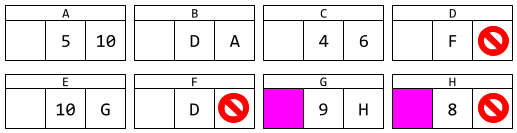
\includegraphics[scale=0.6]{../assets/GCAlg2_1.png}
    \end{center}
    Note that we're only considering non-\code{nil} pairs.

    \item Next, we call \code{mark\_heap} with $B$. This will mark $B$, and then  
    \begin{itemize}
        \item recursively call \code{mark\_heap} with $D$, marking it. Then, we'll recursively call \code{mark\_heap} with $F$, marking it. Finally, we recursively call \code{mark\_heap} with $D$, but since this has already been marked we don't need to do anything.
        
        \begin{center}
            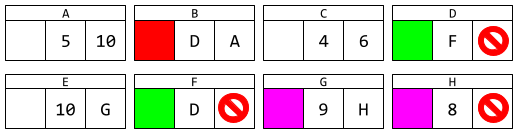
\includegraphics[scale=0.6]{../assets/GCAlg2_2.png}
        \end{center}

        \item after that's done, we cal recursively call \code{mark\_heap} with $A$, marking it. Note that, at $A$, there's no other pairs (only raw numbers), so we're done. 
        
        \begin{center}
            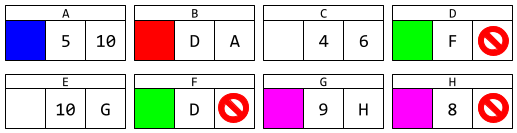
\includegraphics[scale=0.6]{../assets/GCAlg2_3.png}
        \end{center}
    \end{itemize}
\end{itemize}
At this point, we're done. Notice how memory (C) and (E) haven't been marked; this means that they're garbage. Our goal, then, is to move \code{r15} to between $F$ and $G$, and start allocation there! This, however, means we need to move everything back (compacting the heap).


\subsubsection{Step 3: Forward Headers}
\begin{mdframed}
    We'll make use of \code{fwd\_headers}. For each marked pair, this function will set the new address (to store that pair after compating) in the pair's metadata (the first node).
\end{mdframed}

Initially, we'll set \code{move\_to} and \code{move\_from} (\code{to} and \code{from} in the code, respectively) to \code{A} (the first memory location in heap).

\begin{center}
    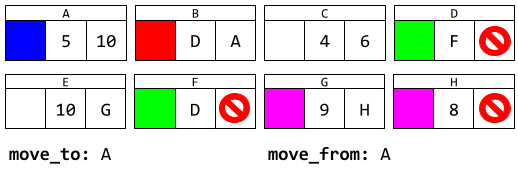
\includegraphics[scale=0.6]{../assets/GCAlg3.png}
\end{center}

Iterating over each block of memory, we have 
\begin{enumerate}
    \item Since $\code{move\_from} = A$ is marked, we set its metadata to $\code{move\_to} = A$ (indicating that we'll move $A$ to $A$ after compacting). We also need to increment \code{move\_to} and \code{move\_from}. This gives us the following diagram: 
    \begin{center}
        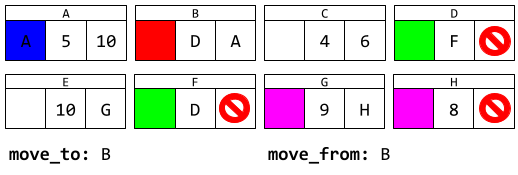
\includegraphics[scale=0.6]{../assets/GCAlg3_1.png}
    \end{center}

    \item Since $\code{move\_from} = B$ is marked, we set its metadata to $\code{move\_to} = B$. We also need to increment \code{move\_to} and \code{move\_from}. This gives us the following diagram: 
    \begin{center}
        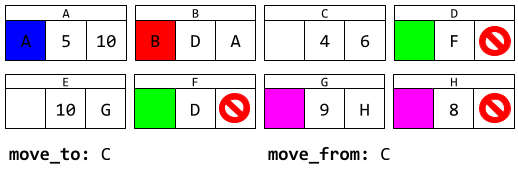
\includegraphics[scale=0.6]{../assets/GCAlg3_2.png}
    \end{center}

    \item Since $\code{move\_from} = C$ is \textbf{not} marked, we only increment \code{move\_from}. This gives us the following diagram: 
    \begin{center}
        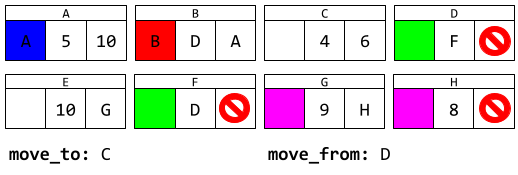
\includegraphics[scale=0.6]{../assets/GCAlg3_3.png}
    \end{center}

    \item Since $\code{move\_from} = D$ is marked, we set its metadata to $\code{move\_to} = C$ (indicating that, after compating, $D$ should be moved to $C$'s location). We also need to increment \code{move\_to} and \code{move\_from}. This gives us the following diagram: 
    \begin{center}
        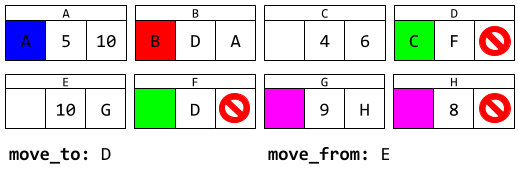
\includegraphics[scale=0.6]{../assets/GCAlg3_4.png}
    \end{center}

    \item Since $\code{move\_from} = E$ is not marked, we only increment \code{move\_from}. This gives us the following diagram: 
    \begin{center}
        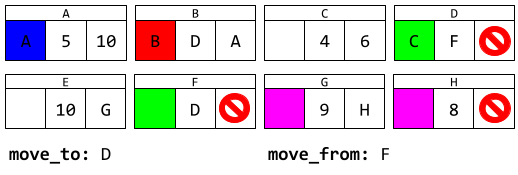
\includegraphics[scale=0.6]{../assets/GCAlg3_5.png}
    \end{center}

    \item Since $\code{move\_from} = F$ is marked, we set its metadata to $\code{move\_to} = D$ (indicating that, after compating, $F$ should be moved to $D$'s location). We also need to increment \code{move\_to} and \code{move\_from}. This gives us the following diagram: 
    \begin{center}
        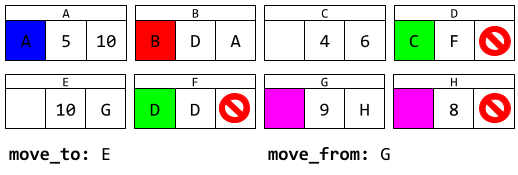
\includegraphics[scale=0.6]{../assets/GCAlg3_6.png}
    \end{center}

    \item Since $\code{move\_from} = G$ is marked, we set its metadata to $\code{move\_to} = E$. We also need to increment \code{move\_to} and \code{move\_from}. This gives us the following diagram: 
    \begin{center}
        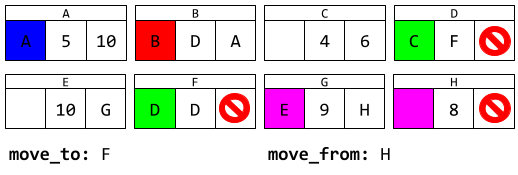
\includegraphics[scale=0.6]{../assets/GCAlg3_7.png}
    \end{center}

    \item Since $\code{move\_from} = H$ is marked, we set its metadata to $\code{move\_to} = F$. We also need to increment \code{move\_to} and \code{move\_from}. This gives us the following diagram: 
    \begin{center}
        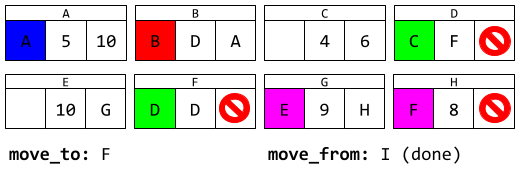
\includegraphics[scale=0.6]{../assets/GCAlg3_8.png}
    \end{center}
\end{enumerate}
At this point, we're done. So, we know where each memory location should be moved to after compactness so that the heap is contiguous. \emph{However}, we still need to update all the internal references within the heap!

\subsubsection{Step 4: Forward Internal Addresses}
\begin{mdframed}
    Now that we've marked where everything should be moved to so we can maintain a contiguous heap structure, we still need to update all internal references so they point to the right places. For this, we'll use \code{fwd\_internal}. The idea is that, for each block of memory, we want to consider each reference that the block has, if any. For each reference $r$: 
    \begin{itemize}
        \item Access the original memory block (before compating) at $r$.
        \item Get its forwarding address and use that as the new reference.
    \end{itemize}
\end{mdframed}
At the moment, this is what our memory diagram looks like: 
\begin{center}
    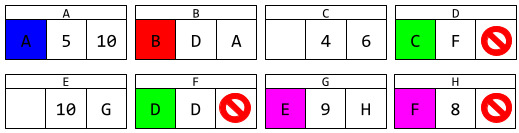
\includegraphics[scale=0.5]{../assets/GCAlg4.png}
\end{center}
\begin{enumerate}
    \item $A$ has no internal references; there's no changes that need to be made. 
    \item One of $B$'s references need to change. 
    \begin{itemize}
        \item Consider reference $D$. Looking up reference $D$, we see that its forwarding address is $C$. Therefore, we replace $D$ with $C$. 
        \item Consider reference $A$. Looking up reference $A$, we see that its forwarding address is $A$. Therefore, we can keep this as $A$. 
    \end{itemize}
    \item $C$ is garbage, so we don't need to consider it. 
    \item For $D$, one of its references need to change. 
    \begin{itemize}
        \item Consider reference $F$. Looking up reference $F$, we see that its forwarding address is $D$. Therefore, we replace $F$ with $D$ here. 
        \item \code{nil} is kept the same. 
    \end{itemize}
    \item $E$ is garbage, so we don't need to consider it. 
    \item One of $F$'s references need to change. 
    \begin{itemize}
        \item Consider reference $D$. Looking it up, we see that its forwarding address is $C$. So, we replace $D$ with $C$.
        \item \code{nil} is kept the same.
    \end{itemize}
    \item One of $G$'s references need to change. 
    \begin{itemize}
        \item 9 is a number, so we leave it alone. 
        \item Consider reference $H$. Looking it up, we see that its forwarding address is $F$. So, we replace $H$ with $F$. 
    \end{itemize}
    \item $H$ has no internal references, so no changes needed.
\end{enumerate}
The result of changing the internal references is 
\begin{center}
    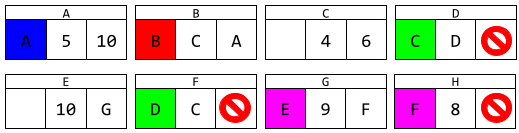
\includegraphics[scale=0.5]{../assets/GCAlg4_1.png}
\end{center}

% more implementation at 28:50

\subsubsection{Step 5: Compacting the Heap}
\begin{mdframed}
    Finally, we want to compact the heap. Compacting will be \emph{iteration} (like \code{fwd\_headers}), \textbf{not} traversal (like \code{mark}). In particular, iteration involves iterating over each live data and copying it to its forwarding pointer.
\end{mdframed}

In the compacting step, we want to 
\begin{itemize}
    \item copy each live data to the forwarding pointer, and 
    \item unmark each data.
\end{itemize}
This gives us 
\begin{center}
    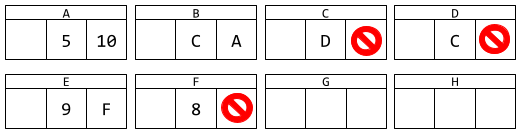
\includegraphics[scale=0.6]{../assets/GCAlg5.png}
\end{center}

\end{document}